\section{Growth}

\begin{multicols}{2}


\subsection{Mitosis Model} % VSO 53

\begin{center}
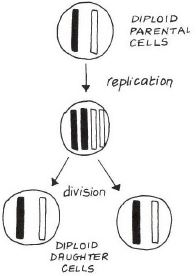
\includegraphics[width=0.3\textwidth]{./img/vso/mitosis-model.jpg}
\end{center}

\begin{description*}
%\item[Subtopic:]{}
\item[Materials:]{Matches or paper strips}
%\item[Setup:]{}
%\item[Procedure:]{}
%\item[Hazards:]{}
%\item[Questions:]{}
%\item[Observations:]{}
\item[Theory:]{In the model shown here, only
one chromosome pair is shown in
the original cell. In a human cell,
one chromosome from the pair
came originally from the sperm,
the other from the ovum. `Parent'
and `daughter' cells have identical
chromosomes.}
%\item[Applications:]{}
\item[Notes:]{The model would be more
realistic and complex if the full
complement of 26 pairs of
chromosomes were used instead
of just one.}
\end{description*}

%==================================================================================================%

\section*{Germination}


\subsection{Seed Germination} % Shika 235 combine see, avocado, potato

%\begin{center}
%\includegraphics[width=0.4\textwidth]{./img/.jpg}
%\end{center}

\begin{description*}
%\item[Subtopic:]{}
\item[Materials:]{Seeds or beans, small bottles, water, avocado pits}
%\item[Setup:]{}
\item[Procedure:]{Cut plastic bottles to make containers. In the first, add soil with beans and water every day. In the second, fill mostly with water and place an avocado seed inside. In the third, fill mostly with water and place a potato inside.}
%\item[Hazards:]{}
%\item[Questions:]{}
\item[Observations:]{The stages of germination can be seen over time.}
\item[Theory:]{The avocado and potato undergo hydroponic germination, since the seed is sprouted by water, air and sunlight only.}
%\item[Applications:]{}
%\item[Notes:]{}
\end{description*}

\columnbreak

\subsection{Conditions for Germination} % LASM 125 PIC!!!

%\begin{center}
%\includegraphics[width=0.4\textwidth]{./img/.png}
%\end{center}

\begin{description*}
%\item[Subtopic:]{}
\item[Materials:]{4 bottles or syringes, cotton wool, beans or seeds, water, oil}
%\item[Setup:]{}
\item[Procedure:]{Place cotton wool at the bottom of each container and add a few beans or seeds to each. In container 1, add enough water to soak the cotton wool. In 2, add cool boiled water to flood the seeds and a small amount of oil. In 3, add ice water. In 4, do not add any water. Record observations over several days.}
%\item[Hazards:]{}
%\item[Questions:]{}
\item[Observations:]{Only container 1 will show proper germination. The others will
show little or no growth because they do not have the conditions necessary
for germination.}
%\item[Theory:]{}
%\item[Applications:]{}
%\item[Notes:]{}
\end{description*}

\subsection{Hypogeal and Epigeal Germination}

\begin{center}
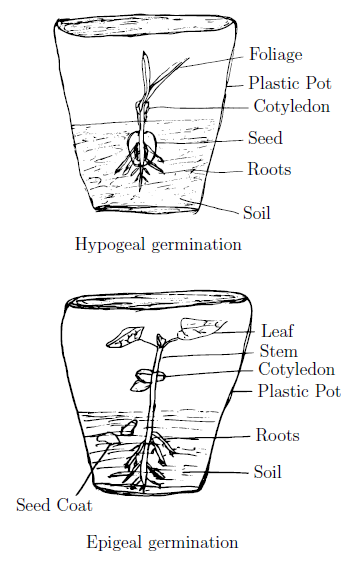
\includegraphics[width=0.35\textwidth]{./img/germination-hyp-ep.png}
\end{center}

\begin{description*}
%\item[Subtopic:]{}
\item[Materials:]{2 pots or bottles, beans, maize seeds}
%\item[Setup:]{}
\item[Procedure:]{Add soil to 2 pots or bottles. Place a few bean seeds in one and a few maize seeds in the other.}
%\item[Hazards:]{}
%\item[Questions:]{}
%\item[Observations:]{}
\item[Theory:]{In epigeal germination cotyledons are carried above the soil, as in the germination of bean seeds (dicotyledonous seeds). In hypogeal germination cotyledons remains underground, as in the germination of maize seeds (monocotyledonous
seeds).}
%\item[Applications:]{}
%\item[Notes:]{}
\end{description*}

%==================================================================================================%


\end{multicols}

\pagebreak